\section{Evaluation}
The evaluation of the clustering algorithms was performed on a Intel i7 1.70 GHz processor (12th gen.) with 16 GB of RAM running Windows 11.

The evaluation of MAFIA was performed using \textit{GPUMAFIA} \cite{gpumafia}, which was installed on a virtual machine (VM) running Ubuntu. The VM was configured with 4 CPUs and 4 GB of RAM.

CLIQUE and SUBCLU were evaluated on the main machine using \textit{ELKI} \cite{elki}. Thus, one should be careful to compare the results of the three algorithms directly, as the execution environment and the implementation may affect the results. However, the growth rate and their clustering of the data sets can be compared.

Throughout the different experiments, a range of input parameters for the three algorithms were tested. The best found were selected. The complete evaluation project can be found in the GitHub repository: \url{https://github.com/henrikdchristensen/SDU-Data-Mining-Exam}. Here, additional experiments as well as detailed descriptions of how to generate the data sets and how to install and use GPUMAFIA is described.

\subsection{Data set generation}
The aim for the synthetic data generation was to be able to produce similar data sets as discussed in \cite{clique,mafia}. That is, hyper-rectangles (axis-parallel) clusters in different subspaces. This was achieved by using \textit{MDCGen}, where different sizes and different densities of the clusters could be determined, as well as which attributes for each cluster that are noise for which values at random is selected from a uniform distribution over the entire range of the attribute.

However, to see the one of the main advantages of SUBCLU compared to CLIQUE and MAFIA, a data set containing a Bezier-shaped cluster was created using \textit{Artificial Cluster} (AC). In addition, a self-populated data set containing a plus-shaped cluster was created as discussed in \cite{mafia}.

Finally, two real-world data sets were selected to evaluate the algorithms in a more realistic setting.

All the data sets were normalized such that each attribute was in the range [0, 1].

\subsection{Experimental Results}

\subsubsection{Scalability with Data Set Size}
To evaluate the scalability of the algorithms a data set containing 20 dimensions with 5 clusters in 5 different subspaces with 10\% noise records was used. The data set size ranges from 10k to 1mio records. The results can be seen in Figure \ref{fig:dataset_size_vs_runtime}. As can be seen, MAFIA is the most scalable algorithm of the three. CLIQUE could handle up to 500k records, while SUBCLU was only able to handle up to 100k records. Similar results in terms of growth rate were reported in all three papers \cite{mafia,clique,subclu}. That is, linear growth for MAFIA and CLIQUE, and quadratic growth for SUBCLU. The linear behaviour of CLIQUE and MAFIA comes from the fact that the number of passes over the data set depends only on the dimensionality of the embedded cluster. An increase in the size of the data set just means that more data has to be scanned on every pass over the data set while finding dense units resulting in a linear growth rate. SUBCLU, on the other hand, has a quadratic growth rate, as it relies on the DBSCAN algorithm which needs partial range queries that can be costly in terms of running time. Better running time of all three is achieved compared to the three papers. This is probably, due to better hardware.

Note that, the \texttt{minpts} in SUBCLU were scaled linearly with the data set size, as the clusters in the dateset were of a fixed size, which means, by increasing the data set size, the density of the clusters increases linearly. However, for the other two algorithms, there was no need to scale any of input parameters, as they relies on the density of the units for the total amount of records.
\begin{figure}[H]
    \vspace*{-0.5cm}
    \centering
    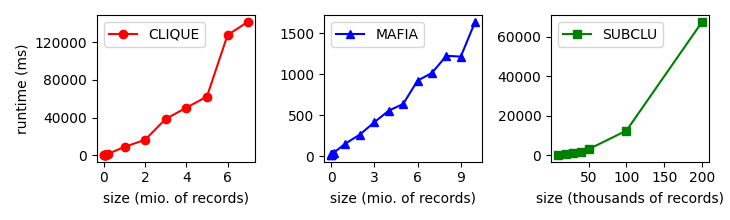
\includegraphics[scale=0.45]{figures/dataset_size_vs_runtime.png}
    \caption{Scalability with increasing data set size.}
    \label{fig:dataset_size_vs_runtime}
    \vspace*{-0.5cm}
\end{figure}

\subsubsection{Clustering Accuracy}
Many different synthetic data sets were generated to test the clustering accuracy of the algorithms.

The first data set were a 2-dimensional data set containing a single cluster formed as a skewed plus-sign with 10\% noise added. Similarly results as in \cite{mafia} was achieved, MAFIA detects the 2-dimensional cluster accurately, whereas CLIQUE finds two overlapping clusters, where none of these detects the borders correctly. The accuracy of MAFIA comes, however, with a cost, as it also reports some lower-dimensional clusters as well.
% The results can be seen in Figure \ref{fig:accuracy_plus}, where only the best cluster found by MAFIA is illustrated. The effect of adaptive grid sizes, clearly shows that MAFIA is more flexible than CLIQUE in such cases.
% \begin{figure}[H]
%     \vspace*{-0.5cm}
%     \centering
%     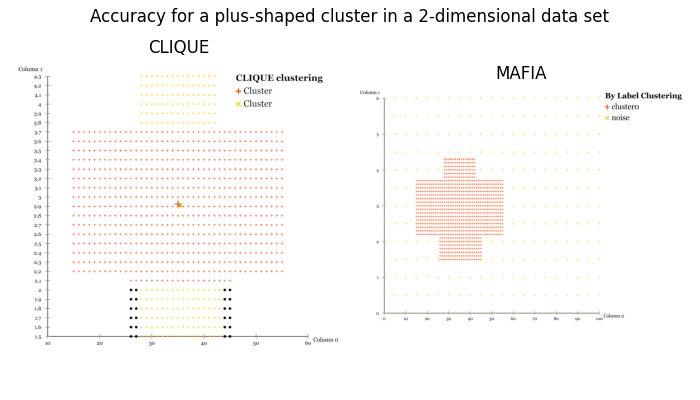
\includegraphics[scale=0.35]{figures/accuracy_plus.png}
%     \caption{A single plus-shaped cluster.}
%     \label{fig:accuracy_plus}
%     \vspace*{-0.5cm}
% \end{figure}

The second data set contains 10 dimensions with contains 2 clusters embedded in a different 4 dimensional subspace. 10\% of the data was added as noise records. Similar data set as the one used in \cite{mafia}. The results can be seen in Figure \ref{fig:accuracy_2clusters}. Here, MAFIA was able to detect the clusters without any additional lower-dimensional clusters. In contrast, CLIQUE reports some overlapping clusters and some of the noise records as clusters. SUBCLU detects also the two clusters, but reports many lower-dimensional clusters and noise records as clusters as well.
\begin{figure}[H]
    \vspace*{-0.5cm}
    \centering
    \subfloat[][CLIQUE]{%
        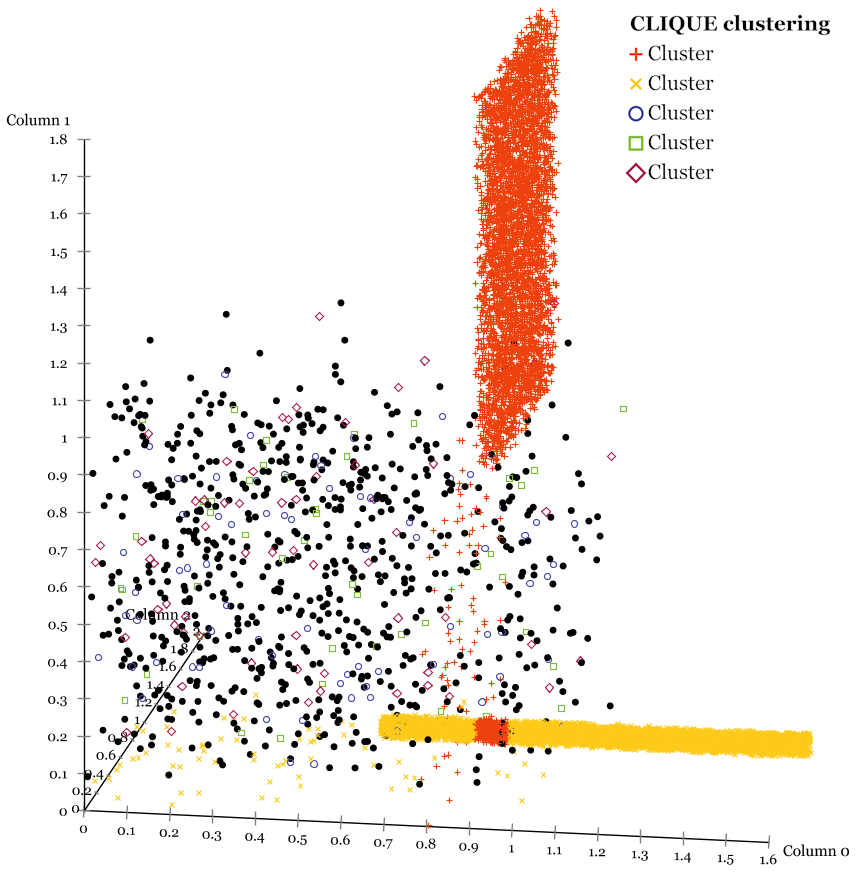
\includegraphics[width=0.3\textwidth]{figures/accuracy_2clusters/clique.png}\label{fig:accuracy_2clusters_clique}}~~~~
    \subfloat[][MAFIA]{%
        \includegraphics[width=0.3\textwidth]{figures/accuracy_2clusters/MAFIA.png}\label{fig:accuracy_2clusters_mafia}}~~~~
    \subfloat[][SUBCLU]{%
        \includegraphics[width=0.3\textwidth]{figures/accuracy_2clusters/SUBCLU.png}\label{fig:accuracy_2clusters_subclu}}
    \caption{Two clusters in 4 different subspaces.}
    \label{fig:accuracy_2clusters}
    \vspace*{-0.5cm}
\end{figure}

The third data set were a 2-dimensional data set containing a single cluster formed as a Bezier curve with 10\% noise added to the data set. As expected, SUBCLU outperforms the other two algorithms as can be seen in Figure \ref{fig:accuracy_bezier}. MAFIA and CLIQUE only partly detects the cluster and reports additional clusters and noise records as clusters. The result of SUBCLU demonstrates its locality assumption and its use of DBSCAN.
\begin{figure}[H]
    \vspace*{-0.5cm}
    \centering
    \subfloat[][CLIQUE]{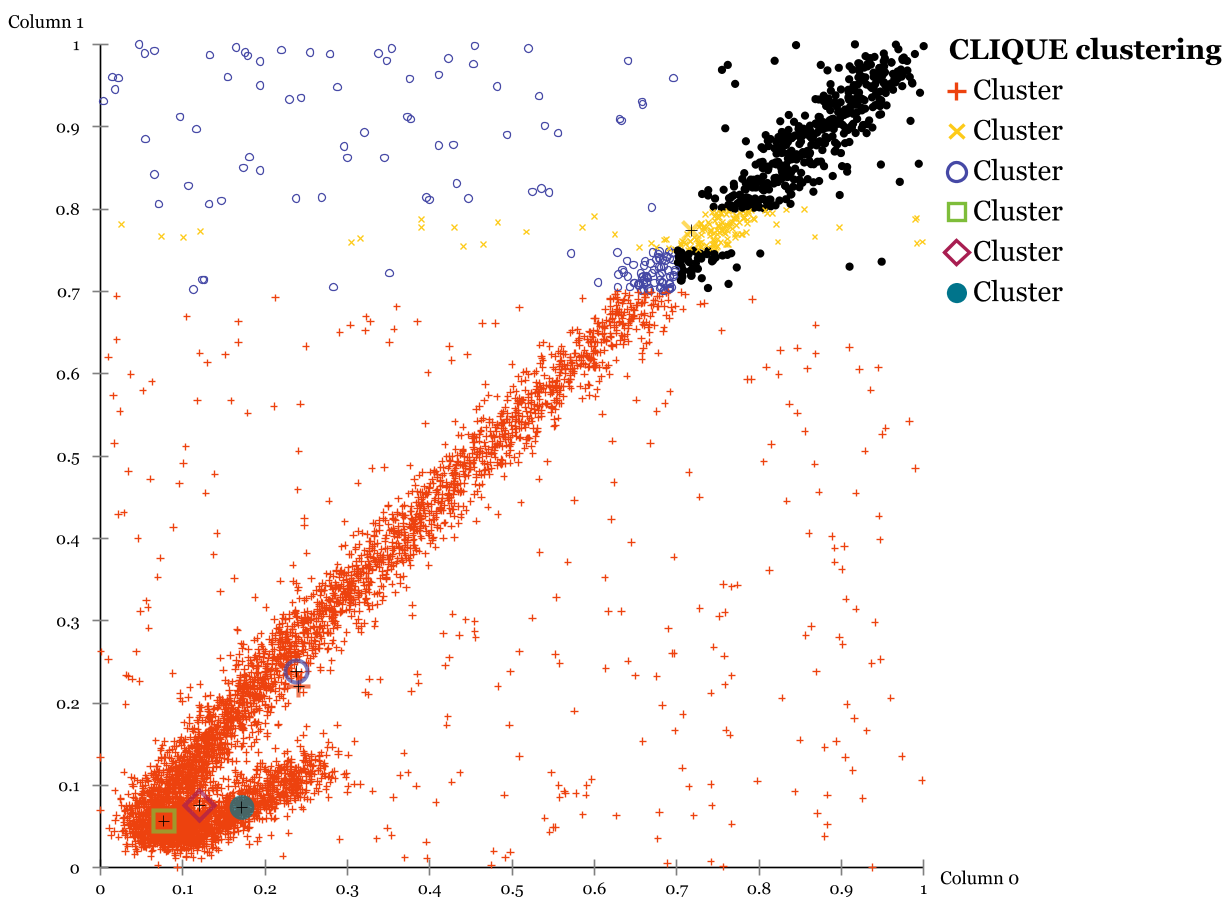
\includegraphics[width=0.3\textwidth]{figures/accuracy_bezier/clique.png}\label{fig:accuracy_bezier_clique}}~~~~
    \subfloat[][MAFIA]{\includegraphics[width=0.3\textwidth]{figures/accuracy_bezier/MAFIA.png}\label{fig:accuracy_bezier_mafia}}~~~~
    \subfloat[][SUBCLU]{\includegraphics[width=0.3\textwidth]{figures/accuracy_bezier/SUBCLU.png}\label{fig:accuracy_bezier_subclu}}
    \caption{A single bezier-shaped cluster.}
    \label{fig:accuracy_bezier}
\end{figure}

\subsubsection{Scalability with Data Dimensionality and Cluster Dimensionality}
Figure \ref{fig:data_dimensionality_vs_runtime} shows the scalability of the CLIQUE and MAFIA with increasing data set dimensionality. The data set contains 1 mio. records with 3 clusters in 5 different subspaces and 10\% noise records, similar to the data set in \cite{mafia}. The data set dimensionality ranges from 10 to 100 dimensions. However, CLIQUE was only able to handle half of the dimensions, as the PC constantly freezes -- probably due to the high memory consumption. In \cite{clique} it is noted that CLIQUE has a quadratic growth rate in terms of data set dimensionality. To investigate this even further, one could try to reduce the memory consumption by having a smaller amount of records in the data set. Nevertheless, MAFIA is the most scalable algorithm of the two.
\begin{figure}[H]
    \vspace*{-0.5cm}
    \centering
    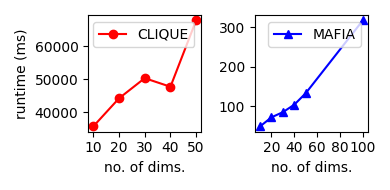
\includegraphics[scale=0.45]{figures/data_dimensionality_vs_runtime.png}
    \caption{Scalability with increasing data set dimensionality.}
    \label{fig:data_dimensionality_vs_runtime}
    \vspace*{-0.5cm}
\end{figure}

Figure \ref{fig:cluster_dimensionality_vs_runtime} shows the scalability of the CLIQUE and MAFIA with increasing cluster dimensionality. A 20-dimensional data set, containing 500k records with a single cluster were used. The cluster was embedded in increasing number of dimensions starting from 10 to 100 dimensions. 10\% of the records was added as noise. The data set is similar to the one used in \cite{mafia}. Both algorithms heavily suffers from the increasing cluster dimensionality, however, MAFIA is able to handle a higher dimensional cluster than CLIQUE. The reason why both algorithms depends on the cluster dimensionality is due to the fact that a higher cluster dimensionality results in a large subspace coverage and a large number of CDUs. In other words, each pass on the data needs to populate a large number of CDUs, adn increase in cluster dimensionality also increases the number of passes over the data set.
\begin{figure}[H]
    \vspace*{-0.5cm}
    \centering
    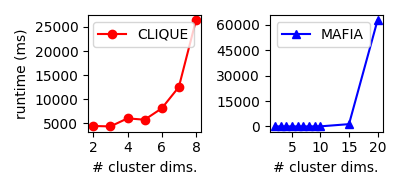
\includegraphics[scale=0.45]{figures/cluster_dimensionality_vs_runtime.png}
    \caption{Scalability with increasing cluster dimensionality.}
    \label{fig:cluster_dimensionality_vs_runtime}
    \vspace*{-0.5cm}
\end{figure}

The results reported for SUBCLU in \cite{subclu} were also tried to be replicated, however, similar it was not possible evaluate in different scales of data set dimensionality and cluster dimensionality, as the PC constantly freezes -- probably due to the high memory consumption. In future work, it would be interesting to investigate this further.

% \subsection{Sensitive analysis for MAFIA}
% From \cite{mafia}, MAFIA should not be sensitive to the choice of $\alpha$. Therefore, a 20-dimensional data set with 1mio data points with 10\% noise were set to evaluate this. $\beta$ was fixed to 35\%, and $\alpha$ was ranging from 0.8 to 5.2 in step size of 0.4. The results can be seen in Figure \ref{fig:sensitivity_alpha}. From the results one could again draw the conclusion that MAFIA is not very sensitive to the $\alpha$ parameter. However, during evaluation of different types of data sets, many different values $\alpha$ was used to detect the right clusters. Also, different $\beta$ values as well as maximum number of windows was needed to be set properly to achieve meaningful results.
% \begin{figure}[H]
%     \vspace*{-0.5cm}
%     \centering
%     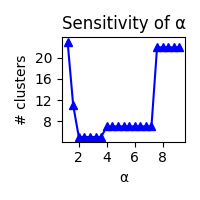
\includegraphics[scale=0.45]{figures/sensitivity_alpha.png}
%     \caption{Sensitivity of $\alpha$ for MAFIA.}
%     \label{fig:sensitivity_alpha}
% \end{figure}

\subsubsection{Real Data Sets}
Two real-world data sets are used to evaluate the algorithms in a more realistic setting. Small data sets were selected for both performance and visualization reasons. Both data sets were normalized such that each attribute was in the range [0, 1].

The first data set is the well-known \textit{Iris} data set \cite{iris}, which contains 150 records of 3 different iris types (e.g. Setosa, Versicolor, Virginica). The data set contains 4 features (sepal length, sepal width, petal length and petal width). All three algorithms produced some meaningful clusters, however, as can be seen in Figure \ref{fig:real_world_iris}. It is hard to determine which algorithm performs the best in this case.
\begin{figure}[H]
    \vspace*{-0.5cm}
    \centering
    \subfloat[][Original]{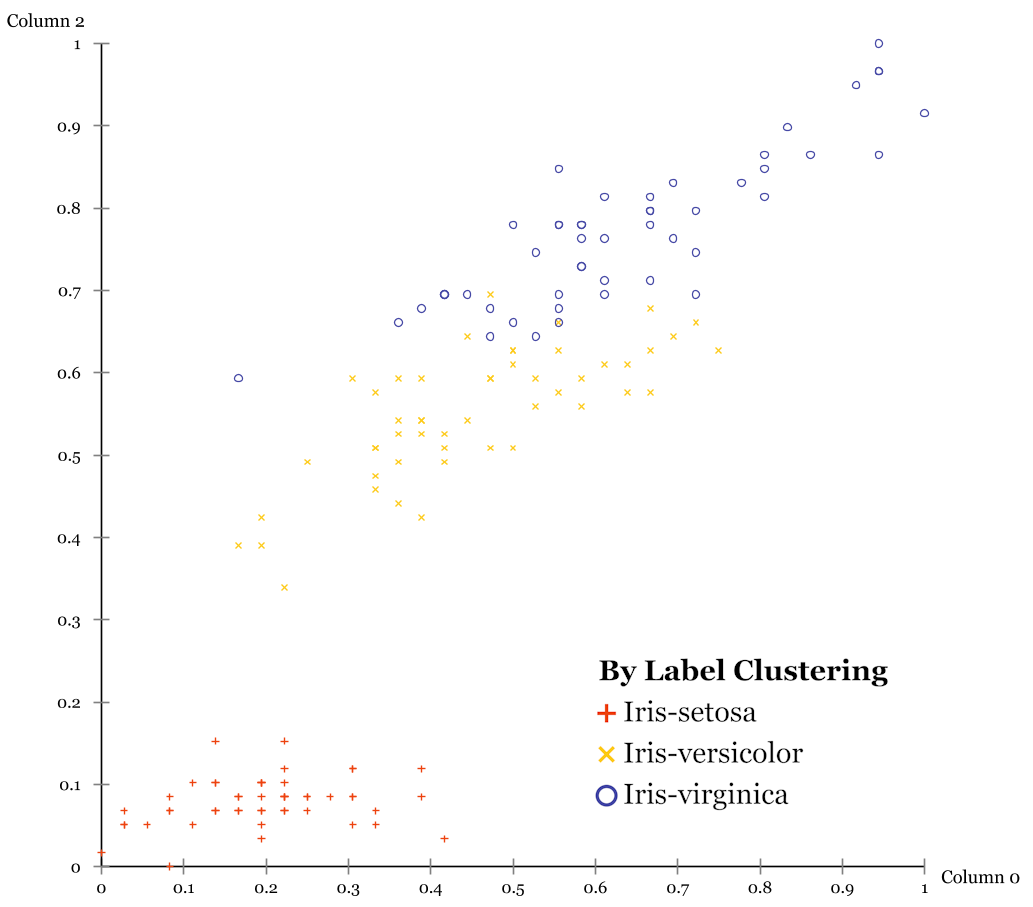
\includegraphics[width=0.3\textwidth]{figures/real_world_iris/orig.png}\label{fig:real_world_iris_orig}}~~~~
    \subfloat[][CLIQUE]{\includegraphics[width=0.3\textwidth]{figures/real_world_iris/CLIQUE.png}\label{fig:real_world_iris_clique}}\\
    \subfloat[][MAFIA]{\includegraphics[width=0.3\textwidth]{figures/real_world_iris/MAFIA.png}\label{fig:real_world_iris_mafia}}~~~~
    \subfloat[][SUBCLU]{\includegraphics[width=0.3\textwidth]{figures/real_world_iris/SUBCLU.png}\label{fig:real_world_iris_subclu}}
    \caption{Iris data set.}
    \label{fig:real_world_iris}
    \vspace*{-0.5cm}
\end{figure}

The second data set is the \textit{Date Fruit} data set \cite{date-fruit}, which contains 898 records of 7 different date fruit types (e.g. Barhee, Deglet Nour, Sukkary, Rotab). These were obtained via a computer vision, where 34 features (e.g shape and color) was extracted. Only SUBCLU were able to produce clusters somewhat close to the true clusters but also finds many lower-dimensional clusters and small clusters. CLIQUE and MAFIA either produced way too many clusters or close to one single cluster.
% \begin{figure}[H]
%     \vspace*{-0.5cm}
%     \centering
%     \subfloat[][Original]{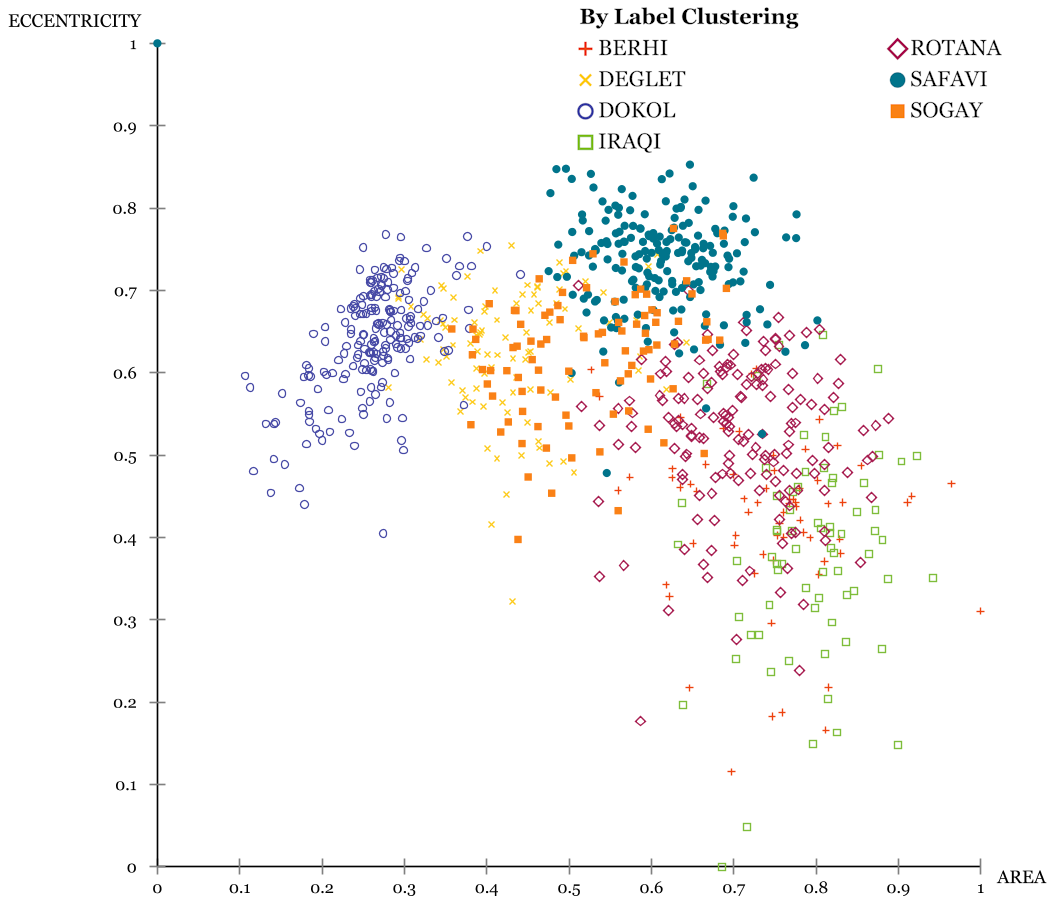
\includegraphics[width=0.3\textwidth]{figures/real_world_date_fruit/orig.png}\label{fig:real_world_date_fruit_orig}}~~~~
%     \subfloat[][SUBCLU]{\includegraphics[width=0.3\textwidth]{figures/real_world_date_fruit/SUBCLU.png}\label{fig:real_world_date_fruit_subclu}}
%     \caption{Date Fruit data set.}
%     \label{fig:real_world_date_fruit}
% \end{figure}